% tesesusp.cls, v-0.1.0

% Based on 'bntex2ppgsi.cls', 'abntex2.csl' and on USP guidelines to create
% thesis and dissertation documents.
% See <https://www.overleaf.com/project/64f7bdf1641ad4a3a8482800>
% and <https://teses.usp.br/index.php?option=com_content&
%      view=article&id=52&Itemid=67&lang=en>
% to learn more.

\clearpage

%:::% class attribute begin/end %:::%

% ----------------------------------------------------------------------
% Cover (mandatory)
% ----------------------------------------------------------------------

%:::% cover body-tag begin %:::%
\imprimircapa
%:::% cover body-tag end %:::%

% ----------------------------------------------------------------------
% Title page (mandatory)
% ----------------------------------------------------------------------

%:::% approval-sheet body-tag begin %:::%
\imprimirfolhaderosto*
%:::% approval-sheet body-tag end %:::%

% ----------------------------------------------------------------------
% Cataloging record (mandatory)
% ----------------------------------------------------------------------

%:::% cataloging-record begin %:::%
\begin{fichacatalografica}
 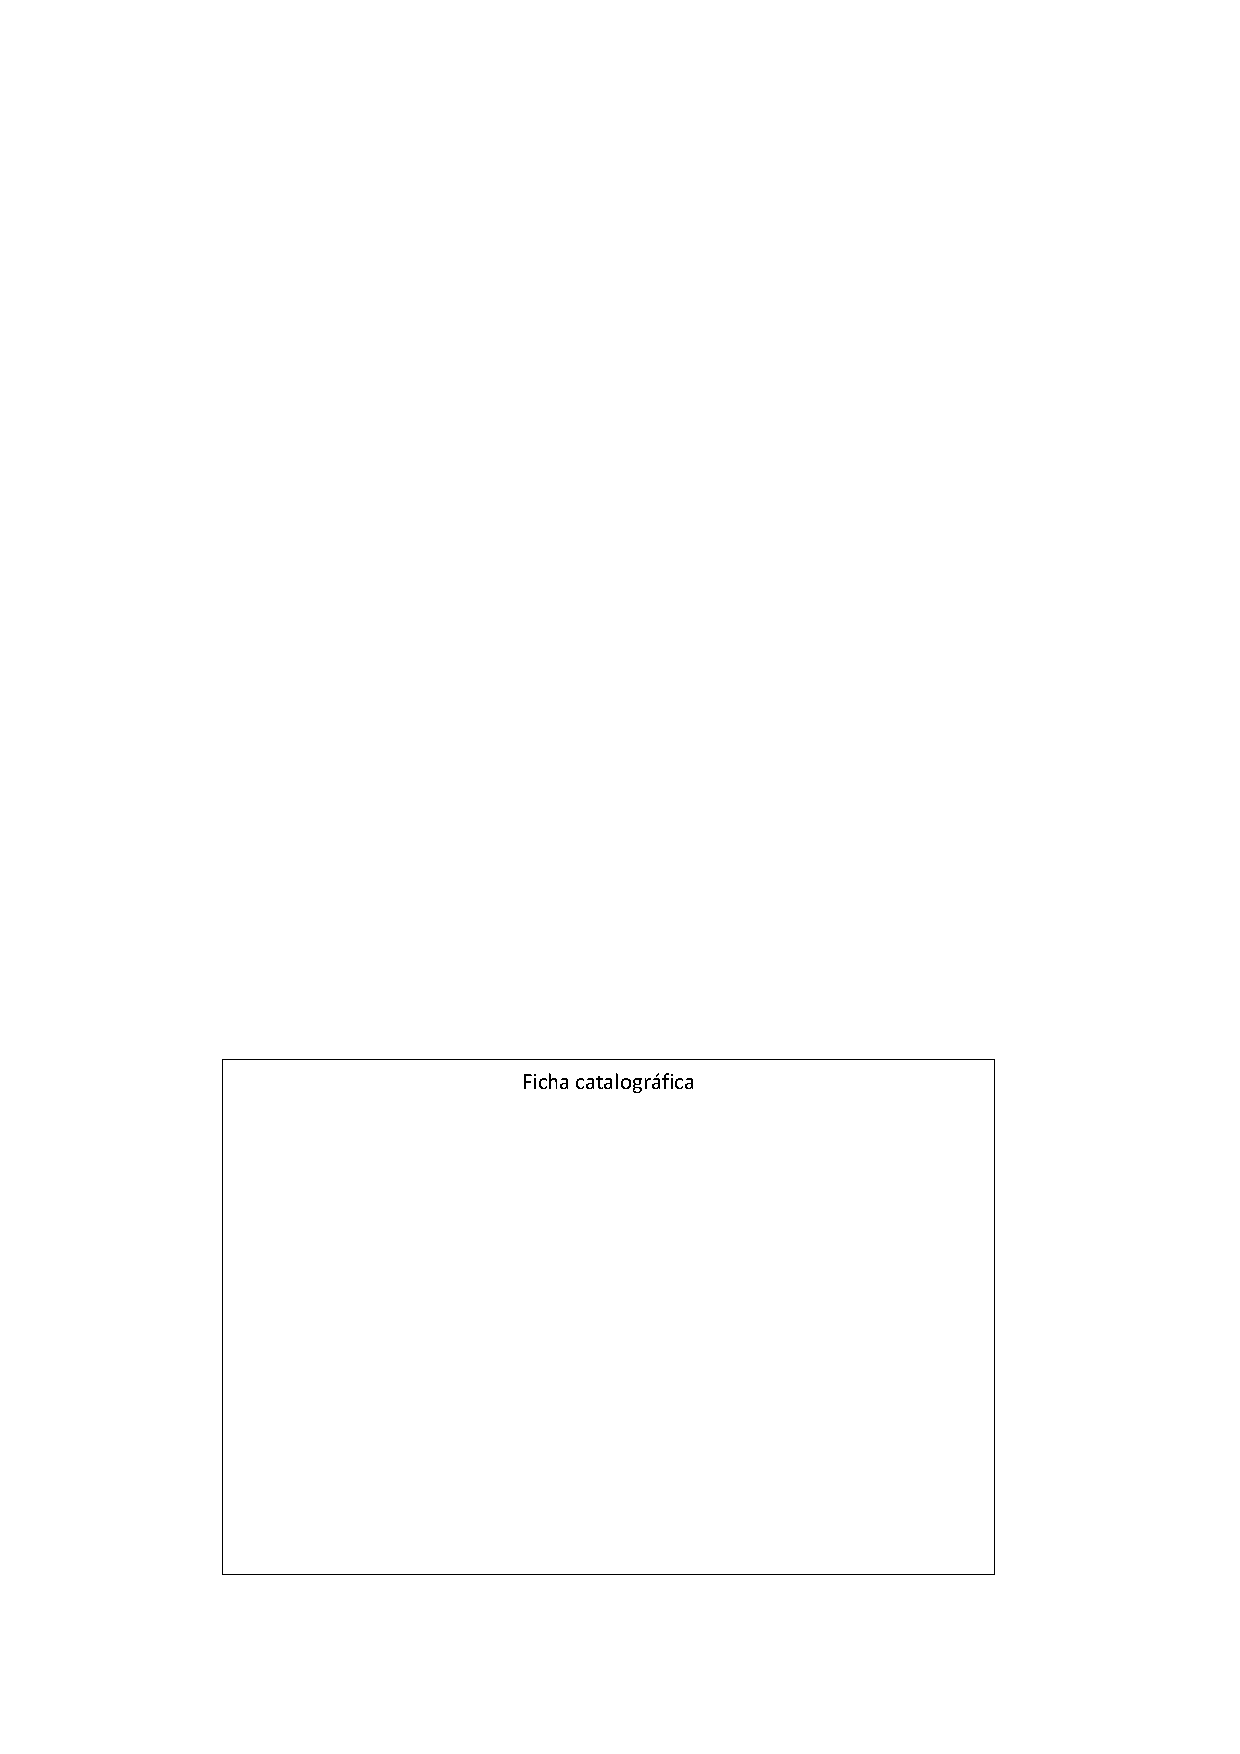
\includepdf{images/fig_ficha_catalografica.pdf}
\end{fichacatalografica}
%:::% cataloging-record end %:::%

% ----------------------------------------------------------------------
% Errata (optional)
% ----------------------------------------------------------------------

%:::% errata begin %:::%
\begin{errata}
  %:::% errata body begin %:::%
This is the development version of the thesis (version \textless1.0.0).
Any necessary corrections will be listed here after its approval.
  %:::% errata body end %:::%
\end{errata}
%:::% errata end %:::%

% ----------------------------------------------------------------------
% Approval sheet (mandatory)
% ----------------------------------------------------------------------

%:::% approval-sheet begin %:::%
\begin{folhadeaprovacao}
  \noindent
  %:::% approval-sheet header begin %:::%
Qualifying exam text by Daniel Vartanian, titled \textbf{Ecology of
sleep and circadian phenotypes of the Brazilian population}, presented
to the School of Arts, Sciences and Humanities at the University of São
Paulo, as part of the requirements for the degree of Master of Science
by the Graduate Program in Modeling Complex Systems (PPG-SCX), in the
concentration area of Fundamentals of Complex Systems.
  %:::% approval-sheet header end %:::%

  \vspace*{1.5cm}

  \noindent
  Approved on \_\_\_\_\_\_\_\_\_\_\_\_\_\_\_\_\_\_\_\_ , \_\_\_\_\_\_\_\_\_\_ .

  \vspace*{1.5cm}

  \begin{center}
    \noindent Examination committee
  \end{center}

  \vspace*{0.5cm}

  \noindent Committee chair:

  \vspace*{0.25cm}

  \renewcommand{\arraystretch}{2}
  \setlength{\arrayrulewidth}{0pt}
  \setlength{\tabcolsep}{0pt}
  \noindent
  \begin{tabular}{m{2cm} P{14cm}}
    Prof. Dr. & \_\_\_\_\_\_\_\_\_\_\_\_\_\_\_\_\_\_\_\_\_\_\_\_\_\_\_\_\_\_\_\_\_\_\_\_\_\_\_\_\_\_\_\_\_\_\_\_\_\_\_\_\_\_\_ \\
    Institution & \_\_\_\_\_\_\_\_\_\_\_\_\_\_\_\_\_\_\_\_\_\_\_\_\_\_\_\_\_\_\_\_\_\_\_\_\_\_\_\_\_\_\_\_\_\_\_\_\_\_\_\_\_\_\_ \\
  \end{tabular}

  \vspace*{1cm}

  \noindent Examiners:

  \vspace*{0.25cm}

  \noindent
  \begin{tabular}{m{2cm} P{14cm}}
    Prof. Dr. & \_\_\_\_\_\_\_\_\_\_\_\_\_\_\_\_\_\_\_\_\_\_\_\_\_\_\_\_\_\_\_\_\_\_\_\_\_\_\_\_\_\_\_\_\_\_\_\_\_\_\_\_\_\_\_ \\
    Institution & \_\_\_\_\_\_\_\_\_\_\_\_\_\_\_\_\_\_\_\_\_\_\_\_\_\_\_\_\_\_\_\_\_\_\_\_\_\_\_\_\_\_\_\_\_\_\_\_\_\_\_\_\_\_\_ \\
    Evaluation & \_\_\_\_\_\_\_\_\_\_\_\_\_\_\_\_\_\_\_\_\_\_\_\_\_\_\_\_\_\_\_\_\_\_\_\_\_\_\_\_\_\_\_\_\_\_\_\_\_\_\_\_\_\_\_ \\
  \end{tabular}

  \vspace*{0.5cm}

  \noindent
  \begin{tabular}{m{2cm} P{14cm}}
    Prof. Dr. & \_\_\_\_\_\_\_\_\_\_\_\_\_\_\_\_\_\_\_\_\_\_\_\_\_\_\_\_\_\_\_\_\_\_\_\_\_\_\_\_\_\_\_\_\_\_\_\_\_\_\_\_\_\_\_ \\
    Institution & \_\_\_\_\_\_\_\_\_\_\_\_\_\_\_\_\_\_\_\_\_\_\_\_\_\_\_\_\_\_\_\_\_\_\_\_\_\_\_\_\_\_\_\_\_\_\_\_\_\_\_\_\_\_\_ \\
    Evaluation & \_\_\_\_\_\_\_\_\_\_\_\_\_\_\_\_\_\_\_\_\_\_\_\_\_\_\_\_\_\_\_\_\_\_\_\_\_\_\_\_\_\_\_\_\_\_\_\_\_\_\_\_\_\_\_ \\
  \end{tabular}

  \vspace*{0.5cm}

  \noindent
  \begin{tabular}{m{2cm} P{14cm}}
    Prof. Dr. & \_\_\_\_\_\_\_\_\_\_\_\_\_\_\_\_\_\_\_\_\_\_\_\_\_\_\_\_\_\_\_\_\_\_\_\_\_\_\_\_\_\_\_\_\_\_\_\_\_\_\_\_\_\_\_ \\
    Institution & \_\_\_\_\_\_\_\_\_\_\_\_\_\_\_\_\_\_\_\_\_\_\_\_\_\_\_\_\_\_\_\_\_\_\_\_\_\_\_\_\_\_\_\_\_\_\_\_\_\_\_\_\_\_\_ \\
    Evaluation & \_\_\_\_\_\_\_\_\_\_\_\_\_\_\_\_\_\_\_\_\_\_\_\_\_\_\_\_\_\_\_\_\_\_\_\_\_\_\_\_\_\_\_\_\_\_\_\_\_\_\_\_\_\_\_ \\
  \end{tabular}
\end{folhadeaprovacao}
%:::% approval-sheet end %:::%

% ----------------------------------------------------------------------
% Inscription (optional)
% ----------------------------------------------------------------------

%:::% inscription begin %:::%
\begin{dedicatoria}
  \vspace*{\fill}
  \centering
  %:::% inscription body begin %:::%
I dedicate this work to the skeptics, the radicals, the ignorant, the
uncivilized, the subversives, the wild dogs, the irreducibles, the
irreconcilables. To the true engines of change. To the destabilizers,
who possess equal or greater importance than the stabilizers. To those
who act on principle, even knowing that there is no ultimate reward or
any meaning in life.
  %:::% inscription body end %:::%
	\vspace*{\fill}
\end{dedicatoria}
%:::% inscription end %:::%

% ----------------------------------------------------------------------
% Acknowledgments (optional)
% ----------------------------------------------------------------------

%:::% acknowledgments begin %:::%
\begin{agradecimentos}
  %:::% acknowledgments body begin %:::%
I would like to acknowledge the following persons and organizations:

Salete Perroni (Sal), my partner in life and in the fight for a better
world.

My Mother, for her unconditional love.

My sister and my brother, for their love and companionship in life.

My friends in science,
\href{https://orcid.org/0000-0003-0004-4487}{Alicia Rafaelly Vilefort
Sales}, \href{https://orcid.org/0000-0002-8222-5240}{Juliana Viana
Mendes}, and \href{https://orcid.org/0000-0002-9283-9967}{Maria Augusta
Medeiros de Andrade}.

My friend and Professor
\href{https://orcid.org/0000-0002-1164-2055}{Humberto Miguel Garay
Malpartida}, for his support; for his principles; and for his integrity,
which was demonstrated when the need arose.

Professor \href{https://orcid.org/0000-0001-6783-6695}{Camilo Rodrigues
Neto}, for introducing me to and teaching me about the science of
complex systems since 2012; for guiding my dissertation; for the
patience and the virtue in taking on and mediating the process of
transitioning my guidance in my master's degree after the breakdown of
relations with my former supervisor.

Professor \href{https://orcid.org/0000-0003-2916-4415}{Carlos Molina
Mendes}, for the speed, impartiality, patience, and virtue in mediating
the process of transitioning my guidance in my master's degree.

My fellow friends: Alex Azevedo Martins; Amanda Moreira; Augusto Amado,
Carina (Cacau) Prado; Cauê Teles; Ítalo Alves Bezerra do Nascimento;
Júlia Mafra; Leonardo Kazuhiko Kawazoe; Letícia Nery de Figueiredo; and
Reginaldo Noveli.

\href{https://lula.com.br/}{President Lula} (Yes!), who saved Brazil
from fascism and approved the long-overdue adjustments to postgraduate
scholarships.

The local student movements, which truly support their category.

The \href{https://prip.usp.br/apoio-estudantil/}{Support Program for
Student Permanence and Education (PAPFE)} of USP, which enabled me to
get this far.

The \href{https://www.gov.br/capes/}{Coordination for the Improvement of
Higher Education Personnel (CAPES)}, for funding this work and enabling
my presence in postgraduate studies.
  %:::% acknowledgments body end %:::%
\end{agradecimentos}
%:::% acknowledgments end %:::%

% ----------------------------------------------------------------------
% Epigraph (optional)
% ----------------------------------------------------------------------

%:::% epigraph begin %:::%
\begin{epigrafe}
  \vspace*{\fill}
	\begin{flushright}
	  %:::% epigraph body begin %:::%
\emph{Nullius in verba}

(The Royal Society, n.d.)
		%:::% epigraph body end %:::%
	\end{flushright}
\end{epigrafe}
%:::% epigraph end %:::%

% ----------------------------------------------------------------------
% Abstract in the vernacular language (mandatory)
% ----------------------------------------------------------------------

%:::% vernacular-abstract begin %:::%
\setlength{\absparsep}{18pt}
\begin{resumo}
  %:::% vernacular-abstract body begin %:::%
Vartanian, D. (2023). \emph{Ecology of sleep and circadian phenotypes of
the Brazilian population} {[}Master's thesis{]}. School of Arts,
Sciences and Humanities, University of São Paulo, São Paulo.
\url{https://danielvartan.github.io/mastersthesis/}

The text below is related to the \textbf{project} of this thesis. The
final abstract can only be produced when the research is completed.

Theories related to sleep and circadian rhythms are already
well-established in science. However, it is necessary to verify and test
these same theories in more extensive samples to obtain a more accurate
picture of the ecology of sleep and temporal phenotypes. This thesis
undertakes this commitment, with the aim of mapping the expression of
sleep-wake cycles and circadian phenotypes in the Brazilian adult
population and investigating the hypothesis that latitude is associated
with circadian rhythm regulation. The latitude hypothesis is based on
the idea that regions located at latitudes near the poles have, on
average, a lower annual incidence of sunlight compared to regions near
the equator (latitude 0°). Therefore, it is deduced that regions near
the equator have a stronger solar zeitgeber, which, according to
chronobiology theories, could lead to a greater propensity for the
synchronization of circadian rhythms in these populations, reducing the
amplitude and diversity of circadian phenotypes. This would also give
these populations a morning characteristic when compared to populations
living far from the equator. To achieve the aforementioned objectives,
this thesis project will rely on a data sample of sleep-wake cycle
expression in the Brazilian population, composed of \(120,265\)
respondents covering all Brazilian states. This data was obtained in
2017 and is based on the Munich ChronoType Questionnaire (MCTQ), a
widely validated questionnaire used to measure circadian phenotypes
based on the sleep-wake cycle expression of individuals in their last
four weeks. The results will contribute to the validation of
chronobiology theories and will generate greater knowledge about the
regulation of circadian rhythms and sleep-wake cycles in the Brazilian
population.

Keywords: chronobiology. chronotype. circadian phenotypes. sleep.
sleep-wake cycle. entrainment. latitude. ecology. mctq.
  %:::% vernacular-abstract body end %:::%
\end{resumo}
%:::% vernacular-abstract end %:::%

% ----------------------------------------------------------------------
% Abstract in the foreign language (mandatory)
% ----------------------------------------------------------------------

%:::% foreign-abstract begin %:::%
\begin{resumo}[RESUMO]
  \begin{otherlanguage*}{brazil}
    %:::% foreign-abstract body begin %:::%
Vartanian, D. (2023). \emph{Ecologia do sono e de fenótipos circadianos
da população brasileira} {[}Dissertação de Mestrado{]}. Escola de Artes,
Ciências e Humanidades, Universidade de São Paulo, São Paulo.
\url{https://danielvartan.github.io/mastersthesis/}

O texto abaixo está relacionado ao \textbf{projeto} desta dissertação. O
resumo final só poderá ser produzido quando a pesquisa for finalizada.

Teorias relacionadas ao sono e aos ritmos circadianos já estão bem
consolidadas na ciência. No entanto, é necessário verificar e testar
essas mesmas teorias em amostras mais abrangentes para obter um retrato
mais preciso da ecologia do sono e dos fenótipos temporais. Esta
dissertação assume esse compromisso, tendo como objetivo mapear a
expressão dos ciclos de sono-vigília e dos fenótipos circadianos da
população adulta brasileira e investigar a hipótese de que a latitude
está associada à regulação do ritmo circadiano. A hipótese da latitude
se fundamenta na ideia de que regiões localizadas em latitudes próximas
aos polos apresentam, em média, uma menor incidência de luz solar anual
quando comparadas com regiões próximas da linha do equador (latitude
0°). Dessa forma, deduz-se que as regiões próximas ao equador apresentam
um zeitgeber solar mais forte, o que, de acordo com as teorias da
cronobiologia, pode gerar uma maior propensão à sincronização dos ritmos
circadianos dessas populações, reduzindo a amplitude e a diversidade de
fenótipos circadianos. Isso também daria a essas populações uma
característica matutina quando comparadas com populações que vivem
distantes da linha do equador. Para atingir os objetivos mencionados, o
projeto irá contar com uma amostra de dados da expressão do ciclo
sono-vigília da população brasileira composta por \(120.265\)
respondentes que abrange todos os estados brasileiros. Essa amostra de
dados foi obtida no ano de 2017 e se baseia no Munich ChronoType
Questionnaire (MCTQ), um questionário amplamente validado e utilizado
para mensurar fenótipos circadianos a partir da expressão do ciclo
sono-vigília de indivíduos em suas últimas quatro semanas. Os resultados
irão contribuir com a validação de teorias da cronobiologia e gerar
conhecimento sobre a regulação do ritmo circadiano e dos ciclos de
sono-vigília da população brasileira.

Palavras-chaves: cronobiologia. cronotipo. fenótipos circadianos. sono.
ciclo sono-vigília. entrainment. latitude. ecologia. mctq.
    %:::% foreign-abstract body end %:::%
  \end{otherlanguage*}
\end{resumo}
%:::% foreign-abstract end %:::%

% ----------------------------------------------------------------------
% List of figures (optional)
% ----------------------------------------------------------------------

%:::% list-of-figures begin %:::%
\setlength{\absparsep}{12pt}
\renewcommand{\listfigurename}{LIST OF FIGURES}
\pdfbookmark[0]{\listfigurename}{lof}
\listoffigures*
\cleardoublepage
%:::% list-of-figures end %:::%

% ----------------------------------------------------------------------
% List of tables (optional)
% ----------------------------------------------------------------------

%:::% list-of-tables begin %:::%
\setlength{\absparsep}{12pt}
\renewcommand{\listtablename}{LIST OF TABLES}
\pdfbookmark[0]{\listtablename}{lot}
\listoftables*
\cleardoublepage
%:::% list-of-tables end %:::%

% ----------------------------------------------------------------------
% List of abbreviations and acronyms (optional)
% ----------------------------------------------------------------------

%:::% list-of-abbreviations begin %:::%
\setlength{\absparsep}{12pt}
\begin{siglas}
  %:::% list-of-abbreviations body begin %:::%
\begin{description}
\item[\textsubscript{F}]
\hspace{20cm}

Subscript indicating a relation with work-free days
\item[\textsubscript{W}]
\hspace{20cm}

Subscript indicating a relation with workdays
\item[BT]
\hspace{20cm}

Local time of going to bed
\item[FD]
\hspace{20cm}

Number of work-free days per week
\item[GU]
\hspace{20cm}

Local time of getting out of bed
\item[HO]
\hspace{20cm}

Horne \& Ostberg's morningness-eveningness questionnaire (same as
\emph{MEQ})
\item[LE]
\hspace{20cm}

Light exposure
\item[LE\textsubscript{week}]
\hspace{20cm}

Average weekly light exposure
\item[MCTQ]
\hspace{20cm}

Munich ChronoType Questionnaire
\item[MCTQ\textsuperscript{PT}]
\hspace{20cm}

Portuguese version of the MCTQ
\item[MEQ]
\hspace{20cm}

Morningness-Eveningness Questionnaire
\item[MSF]
\hspace{20cm}

Local time of mid-sleep on work-free days
\item[MSF\textsubscript{sc}]
\hspace{20cm}

Chronotype proxy. The midpoint between sleep onset and sleep end on
work-free days. A sleep correction (\textsubscript{SC}) is made when a
possible sleep compensation related to a lack of sleep on workdays is
identified.
\item[MSW]
\hspace{20cm}

Local time of mid-sleep on workdays
\item[PRC]
\hspace{20cm}

Phase response curve
\item[SD]
\hspace{20cm}

Sleep duration
\item[SD\textsubscript{week}]
\hspace{20cm}

Average weekly sleep duration
\item[SE]
\hspace{20cm}

Local time of sleep end
\item[SI]
\hspace{20cm}

``Sleep inertia''. Despite the name, this abbreviation represents the
time that a person takes to get up after sleep end. It is used this way
by the MCTQ authors.
\item[SJL]
\hspace{20cm}

Absolute social jetlag
\item[SJL\textsubscript{rel}]
\hspace{20cm}

Relative social jetlag
\item[SJL\textsubscript{sc}]
\hspace{20cm}

Jankowski's sleep-corrected social jetlag
\item[SJL\textsubscript{sc-rel}]
\hspace{20cm}

Jankowski's relative sleep-corrected social jetlag
\item[Sloss\textsubscript{week}]
\hspace{20cm}

Weekly sleep loss
\item[SO]
\hspace{20cm}

Local time of sleep onset
\item[Slat]
\hspace{20cm}

Sleep latency, i.e., time (duration) to fall asleep after deciding to
sleep
\item[SPrep]
\hspace{20cm}

Local time of preparing to sleep
\item[TBT]
\hspace{20cm}

Total time in bed
\item[WD]
\hspace{20cm}

Number of workdays per week
\end{description}
  %:::% list-of-abbreviations body end %:::%
\end{siglas}
%:::% list-of-abbreviations end %:::%

% ----------------------------------------------------------------------
% List of symbols (optional)
% ----------------------------------------------------------------------

%:::% list-of-symbols begin %:::%
\setlength{\absparsep}{12pt}
\begin{simbolos}
  %:::% list-of-symbols body begin %:::%
For an extensive list of chronobiology related symbols, please refer to
Aschoff et al.~(1965) and Marques \& Oda (2012).

\begin{description}
\item[\(\tau\)]
\hspace{20cm}

Period of a rhythm in free flow. Only revealed under constant
environmental conditions.
\item[\(T\)]
\hspace{20cm}

Zeitgeber period
\item[\(\phi\)]
\hspace{20cm}

Phase
\item[\(\Delta\phi\)]
\hspace{20cm}

Phase shift
\item[\(+\Delta\phi\)]
\hspace{20cm}

Phase advance
\item[\(-\Delta\phi\)]
\hspace{20cm}

Phase delay
\item[\(\Psi\)]
\hspace{20cm}

Phase relation
\end{description}
  %:::% list-of-symbols body end %:::%
\end{simbolos}
%:::% list-of-symbols end %:::%

% ----------------------------------------------------------------------
% List of terms and definitions (optional)
% ----------------------------------------------------------------------

%:::% list-of-terms begin %:::%
\setlength{\absparsep}{12pt}
\begin{termos}
  %:::% list-of-terms body begin %:::%
For an extensive list of chronobiology related terms and definitions,
please refer to Aschoff et al.~(1965) and Marques \& Oda (2012).

\begin{description}
\item[Chronotype]
\hspace{20cm}

Any kind of temporal phenotype (Ehret, 1974; Pittendrigh, 1993).
Usually, it refers to circadian phenotypes in a spectrum that goes from
morningness to eveningness (Horne \& Ostberg, 1976; Roenneberg et al.,
2003). It can also be seen as an organism's phase of entrainment
(Roenneberg et al., 2012).
\end{description}

\begin{description}
\item[Circadian rhythm]
\hspace{20cm}

A rhythm with a period close to a day/24h, an approximation to the
period of the earth's rotation (Pittendrigh, 1960). From the Latin
\emph{circā}, around, and \emph{dĭes}, day (Latinitium, n.d.). Example:
the sleep-wake cycle.
\end{description}

\begin{description}
\item[Complex system]
\hspace{20cm}

There are several definitions. Here are some that I found to be of use:
\end{description}

\begin{itemize}
\tightlist
\item
  ``Systems that don't yield to compact forms of representation or
  description'' (David Krakauer apud Mitchell, 2013)
\item
  ``A system of many interacting parts where the system is more than
  just the sum of its parts'' (Mark Newman apud Mitchell, 2013)
\item
  Systems with many connected agents that interact and exhibit
  self-organization and emergence behavior, all without the need for a
  central controller (adapted from Camilo Rodrigues Neto's definition,
  supervisor of this thesis).
\item
  Dialectics at its finest (my working definition).
\end{itemize}

\begin{description}
\item[Entrainment]
\hspace{20cm}

A shift and alignment of biological rhythms induced by a zeitgeber input
(Kuhlman et al., 2018). For example: a shift/alignment of an organism's
circadian rhythm when exposed to light.
\end{description}

\begin{description}
\item[Infradian rhythm]
\hspace{20cm}

A rhythm with a period greater than a day/24h. From the Latin
\emph{infrā}, below (think in terms of period repetition), and
\emph{dĭes}, day (Latinitium, n.d.). Example: the menstrual cycle.
\end{description}

\begin{description}
\item[Period]
\hspace{20cm}

Cycle duration of an oscillation. In a more technical way, the duration
between two identical and consecutive phases in an oscillation (Kuhlman
et al., 2018).
\end{description}

\begin{description}
\item[System theory]
\hspace{20cm}

Two definitions can be of use:
\end{description}

\begin{itemize}
\tightlist
\item
  Science or discipline that investigates models, principles, and laws
  that are valid to systems in general (Bertalanffy, 1968)
\item
  ``The attempt of a reductionist scientific tradition to come to terms
  with complexity, nonlinearity, and change through sophisticated
  mathematical and computational techniques, \emph{a groping toward a
  more dialectical understanding} that is held back by its philosophical
  biases and the institutional and economic contexts of its
  development'' (Levins, 1998)
\end{itemize}

\begin{description}
\item[Ultradian rhythm]
\hspace{20cm}

A rhythm with a period below a day/24h. From the Latin \emph{ultrā},
beyond (think in terms of period repetition), and \emph{dĭes}, day
(Latinitium, n.d.). Example: the cardiac cycle.
\end{description}

\begin{description}
\item[Zeitgeber]
\hspace{20cm}

Any periodic environmental signal/cue that can influence or regulate
biological rhythms. From the German \emph{zeit}, time, and \emph{geber},
donor (Cambridge University Press, n.d.). Two main well known zeitgebers
are light exposure and environment temperature (Pittendrigh, 1960).
\end{description}
  %:::% list-of-terms body end %:::%
\end{termos}
%:::% list-of-terms end %:::%

% ----------------------------------------------------------------------
% Table of contents (mandatory)
% ----------------------------------------------------------------------

%:::% table-of-contents begin %:::%
\setlength{\absparsep}{12pt}
\renewcommand{\contentsname}{TABLE OF CONTENTS}
\pdfbookmark[0]{\contentsname}{toc}
% \tableofcontents*
\cleardoublepage
%:::% table-of-contents end %:::%
